% !TEX root = ../MasterThesis_goto_v1.tex

%%%%%%%%%%%%%%%%%%%%%%%%%%%%%%%%%%%%%%%%%%%%%%%%%%%%%%%%%%%%%%%%%%%%%%%%%%%%%%%%%%%%%%%%%%%%%%%%%%%%%
\chapter{崩壊点検出の為のネットワーク} \label{chap:Networks}

\ref{chap:Networks}章と\ref{chap:VertexFinderwithDL}章、\ref{chap:Comparison}章は本論文の本題である。
\ref{chap:Networks}章では本研究で使用するデータと深層学習のネットワークについて、\ref{chap:VertexFinderwithDL}章では\ref{chap:Networks}章で作成したネットワークを用いた崩壊点検出について、\ref{chap:Comparison}章ではその様にして作成した崩壊点検出と現行の崩壊点検出との比較について、それぞれ解説する。

本章では、まず\ref{Net:Data}節で本研究で取り扱うデータの性質について述べる。
次に、\ref{Net:forVertexFinderwithDL}節にて深層学習を使用した崩壊点検出をどのように実現するかについて概要を説明する。
個々のネットワークの詳細な構造や学習、ネットワーク単体での性能については\ref{Net:PairModel}節、\ref{Net:VertexLSTM}節で解説する。
これらネットワークについては\ref{chap:DeepLearning}章の内容を前提とし、訓練データ、ハイパーパラメータ・チューニングについてもここで述べる。

%%%%%%%%%%%%%%%%%%%%%%%%%%%%%%%%%%%%%%%%%%%%%%%%%%%%%%%%%%%%%%%%%%%%%%%%%%%%%%%%%%%%%%%%%%%%%%%%%%%%%
\section{データ} \label{Net:Data}

ここでは、本研究で使用したモンテカルロシミュレーションデータについて述べる。
特に\ref{Net:Data:DataProperty}項では、データ全体についての性質に関して、\ref{Net:Data:TrackInformationandPreprocessing}項では、本研究で使用する飛跡についての情報と前処理について詳しく述べる。
ただし、各ネットワークの学習に使用する訓練データの詳細に関しては、後の\ref{Net:PM:TrainingandStrategyofPM}や\ref{Net:VLSTM:TrainingandStrategyofVLSTM}で紹介する。

%%%%%%%%%%%%%%%%%%%%%%%%%%%%%%%%%%%%%%%%%%%%%%%%%%%%%%%%%%%%%%%%%%%%%%%%
\subsection{データ全体の性質} \label{Net:Data:DataProperty}

どのようなシミュレーションソフトを使っているか。\\
エネルギー・終状態・Tertiary Vertex・事象毎の飛跡の数・崩壊点の種類と割合・(後述する)本数個数が異なる

%%%%%%%%%%%%%%%%%%%%%%%%%%%%%%%%%%%%%%%%%%%%%%%%%%%%%%%%%%%%%%%%%%%%%%%%
\subsection{飛跡の情報と前処理} \label{Net:Data:TrackInformationandPreprocessing}

各変数について・Helix parametersの定義\cite{TrackParametersLCIO}
Helix parametersの元の分布やreshape後の分布について\\

%%%%%%%%%%%%%%%%%%%%%%%%%%%%%%%%%%%%%%%%%%%%%%%%%%%%%%%%%%%%%%%%%%%%%%%%%%%%%%%%%%%%%%%%%%%%%%%%%%%%%
\section{深層学習を用いた崩壊点検出の実現} \label{Net:forVertexFinderwithDL}

深層学習ができること。分類・回帰問題に落とし込むという事。\\
気をつけねばならないこと。データの性質にあったネットワークが必要である。今回取り扱うデータにおいて、\\

以上を踏まえた上で私は二つのネットワークを用いた崩壊点検出を提案する。\\
一つはを用いて、崩壊点の種類と位置の予測を行う為のネットワークである。\\
もう一つはとを用いて、を行う為のネットワークである。\\
詳細なネットワークの構造については、後の\ref{Net:PairModel}、\ref{Net:VertexLSTM}節で述べる。\\

これらのネットワークはを用いて実装した。\\
tensorflow・keras・TITAN RTX・ITO\\


%%%%%%%%%%%%%%%%%%%%%%%%%%%%%%%%%%%%%%%%%%%%%%%%%%%%%%%%%%%%%%%%%%%%%%%%%%%%%%%%%%%%%%%%%%%%%%%%%%%%%
\section{飛跡対についてのネットワーク} \label{Net:PairModel}

ここでは\ref{Net:forVertexFinderwithDL}節で紹介した二つのネットワークの内、飛跡対についてのネットワークについて述べる。
主にネットワークの構造に関しては\ref{Net:PM:StructureofPM}項で、学習に関しては\ref{Net:PM:TrainingandStrategyofPM}項で解説する。
また、そのようにして構築、訓練されたネットワーク単体についての性能と評価に関しては、\ref{Net:PM:PerformanceofPM}項で述べることとする。

%%%%%%%%%%%%%%%%%%%%%%%%%%%%%%%%%%%%%%%%%%%%%%%%%%%%%%%%%%%%%%%%%%%%%%%%
\subsection{ネットワークの構造} \label{Net:PM:StructureofPM}

飛跡対についてのネットワークは崩壊点の種類を分類するネットワークと崩壊点の位置を予想するネットワークの二つの作成を行なったが、基本的な構造は同一である為、ここでは主に崩壊点の種類を分類するネットワークについての構造のみ解説する。
また、終状態が$c\bar{c}$となるデータについては、非結合な飛跡対・Primary Vertex・フレーバー$c$のSecondary Vertexの3クラス分類であるのに対し、終状態が$b\bar{b}$となるデータについては、非結合な飛跡対・Primary Vertex・フレーバー$b$のSecondary Vertex・フレーバー$c$のSecondary (Tertiary) Vertexの4つとフレーバー$b$のSecondary Vertex由来の飛跡とそこから生じたフレーバー$c$のSecondary Vertex由来の飛跡を一本ずつ含んだ飛跡対の5クラスで分類を行う。

飛跡対についてのネットワークは非常にシンプルな構造のものを使用した。
ネットワークの概略図を図\ref{}に示す。

ここで、過学習 (Over fitting) を避ける為、Batch Normalization\cite{}を全結合層の後ろに入れている。
また勾配消失への対策として、活性化関数は全てReLU関数を使用している。

ノード数や層数に関してのハイパーパラメータ・チューニングに関しては\ref{Net:PM:PerformanceofPM}にて

\begin{figure}[h]
 \centering
 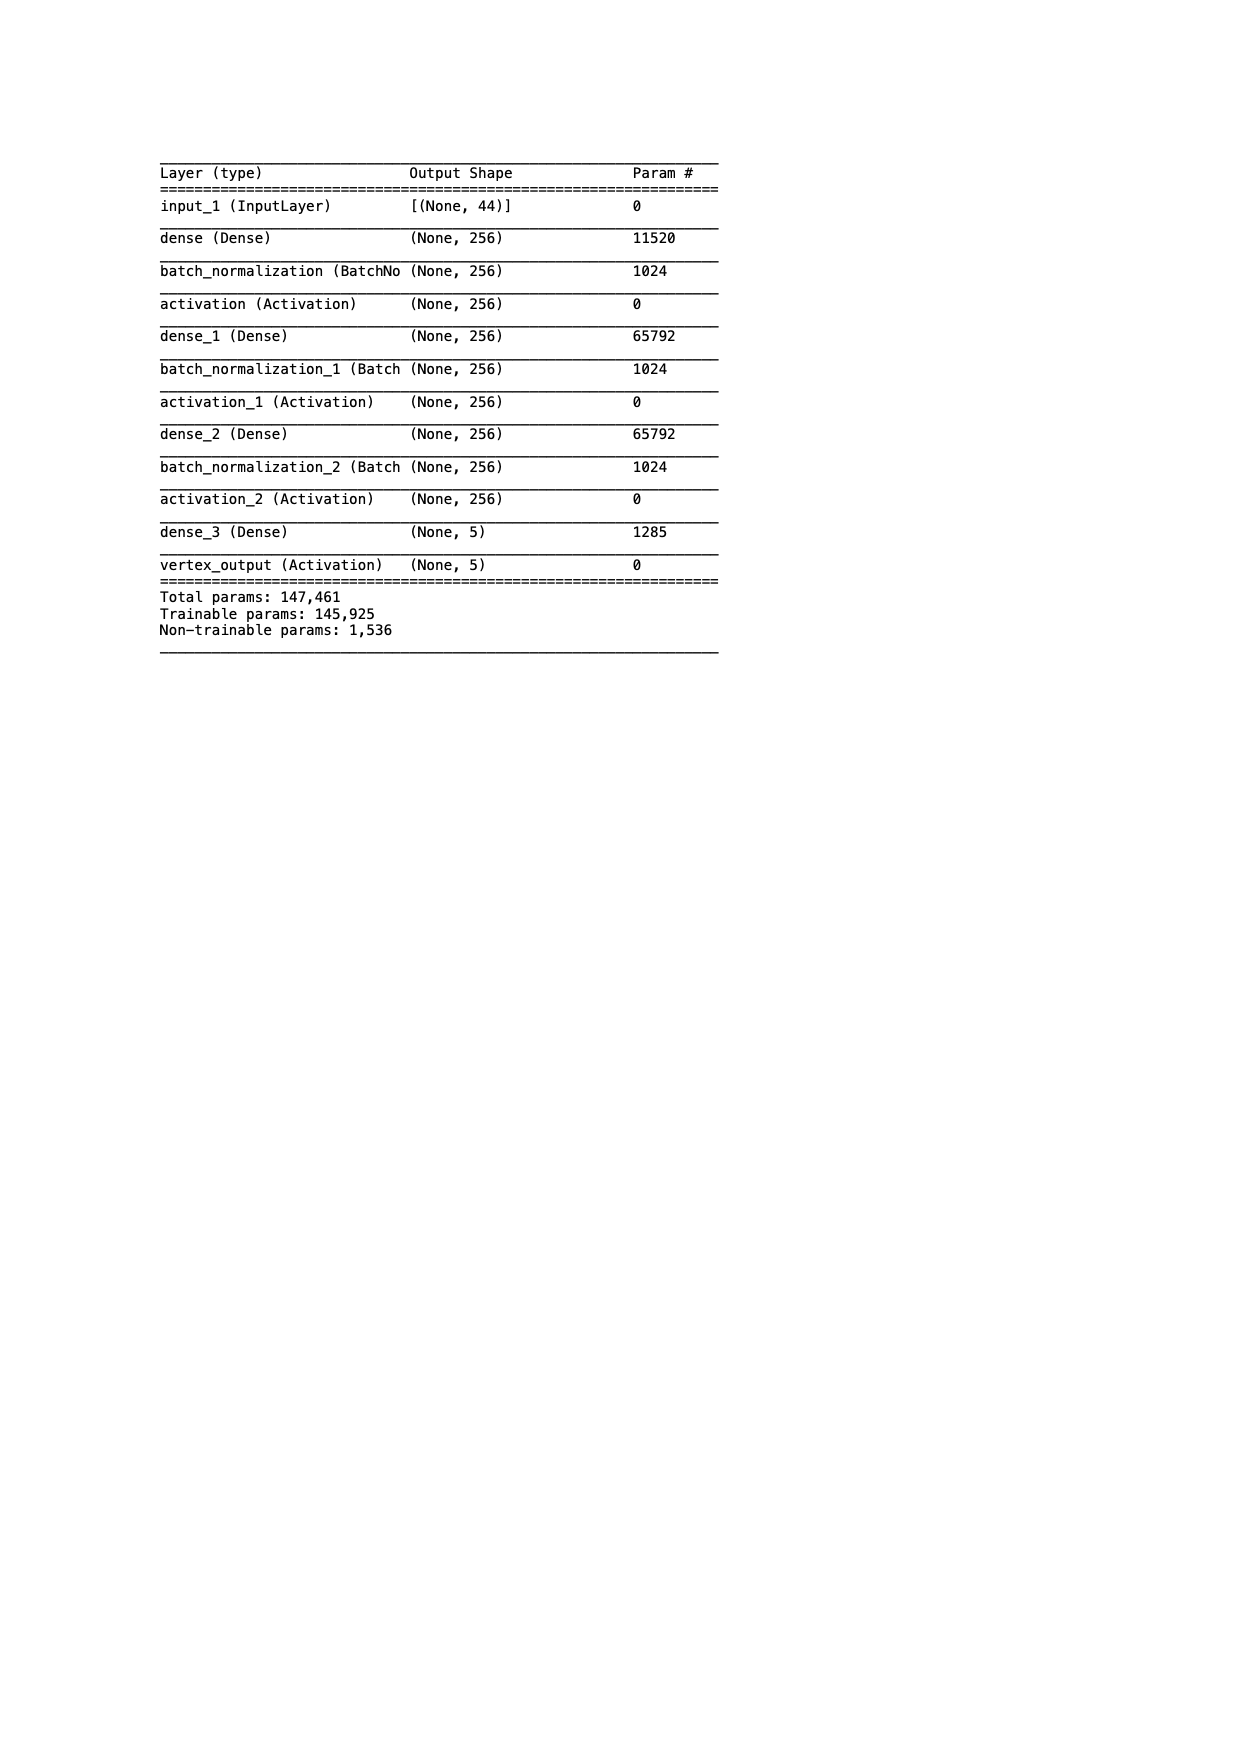
\includegraphics[trim = 75 500 125 0, width=0.9\textwidth]{Figure/3Networks/3-3-1-1PairModelSummary.png}
 \caption{$b\bar{b}$データセットについて崩壊点種予測モデルにおける各種パラメーターの出力}
 \label{3-3-1-1PairModelSummary}
\end{figure}


%%%%%%%%%%%%%%%%%%%%%%%%%%%%%%%%%%%%%%%%%%%%%%%%%%%%%%%%%%%%%%%%%%%%%%%%
\subsection{ネットワークの学習と戦略} \label{Net:PM:TrainingandStrategyofPM}

訓練データ\\
飛跡対は全ての組み合わせを考える・不均衡データ・重みをつけた学習

正答率・Lossのカーブ\\

%%%%%%%%%%%%%%%%%%%%%%%%%%%%%%%%%%%%%%%%%%%%%%%%%%%%%%%%%%%%%%%%%%%%%%%%
\subsection{ネットワークの性能} \label{Net:PM:PerformanceofPM}

ハイパーパラメータ・チューニング\\

位置を見ているか\\
Chi2, Pos, Cov Mat, 位置を予想するネットワーク\\

Othersなクラスを加えた分類\\

ROCカーブ\\


%%%%%%%%%%%%%%%%%%%%%%%%%%%%%%%%%%%%%%%%%%%%%%%%%%%%%%%%%%%%%%%%%%%%%%%%%%%%%%%%%%%%%%%%%%%%%%%%%%%%%
\section{任意の数の飛跡についてのネットワーク} \label{Net:VertexLSTM}

ここでは\ref{Net:forVertexFinderwithDL}節で紹介した二つのネットワークの内、任意の数の飛跡のためのネットワークについて述べる。
基本的には前節の飛跡対についてのネットワークと同様の手順での解説を行うが、この任意の数の飛跡についてのネットワークは、既存のネットワーク構造にはない独自のネットワークで構築している。
これは本研究におけるデータの特殊性や問題解決のための最適なネットワークを考慮した結果である。
このようなネットワークの詳細な構造については\ref{Net:VLSTM:DetailedStructureofVLSTM}項で述べる。


%%%%%%%%%%%%%%%%%%%%%%%%%%%%%%%%%%%%%%%%%%%%%%%%%%%%%%%%%%%%%%%%%%%%%%%%
\subsection{ネットワークの構造} \label{Net:VLSTM:StructureofVLSTM}

任意の数の飛跡についてのネットワークは、飛跡対についてのネットワークによって得られた、崩壊点のタネに対して1事象中の飛跡を一本ずつ繋げていき崩壊点を生成するネットワークである。
したがって、その出力はある飛跡について、その飛跡が崩壊点のタネと結合するか否かの二値分類となる。

この様な次々と飛跡を処理し、逐次崩壊点の情報を更新していくネットワークはリカレントニューラルネットワークを用いる事で作成できる。
ただし、飛跡は系列データではない為、リカレントニューラルネットワークをそのまま用いることはデータの性質に合わない。
この為、私はLSTMを拡張し、新しい独自のリカレントニューラルネットワークの構造を構築した。
この独自のネットワーク構造については、次項\ref{Net:VLSTM:DetailedStructureofVLSTM}にて解説する。
ここでは、より大きな枠組みとしてのネットワークの構造について述べる。

図\ref{3-4-1-1SimpleVLSTM}は、リカレントニューラルネットワークを用いた最も簡単な崩壊点生成を表現したものである。
ここで、左から崩壊点の種である飛跡対が入力されている。
実際には全結合層を通し、リカレントニューラルネットワークの初期状態としている。
この初期状態は、リカレントニューラルネットワーク内の重みと共に全結合層が学習される為、学習可能な初期状態 (Trainable (Learnable) Initial State) となっている。
また、飛跡は下から一本ずつ入力され、1事象分の全ての飛跡が使用されるが、リカレントニューラルネットワークである為、系列として扱う飛跡の本数は任意である。
したがって、ある崩壊点のタネに対して、任意の数の飛跡が結合しているか否かを分類することができる。

\begin{figure}[h]
 \centering
 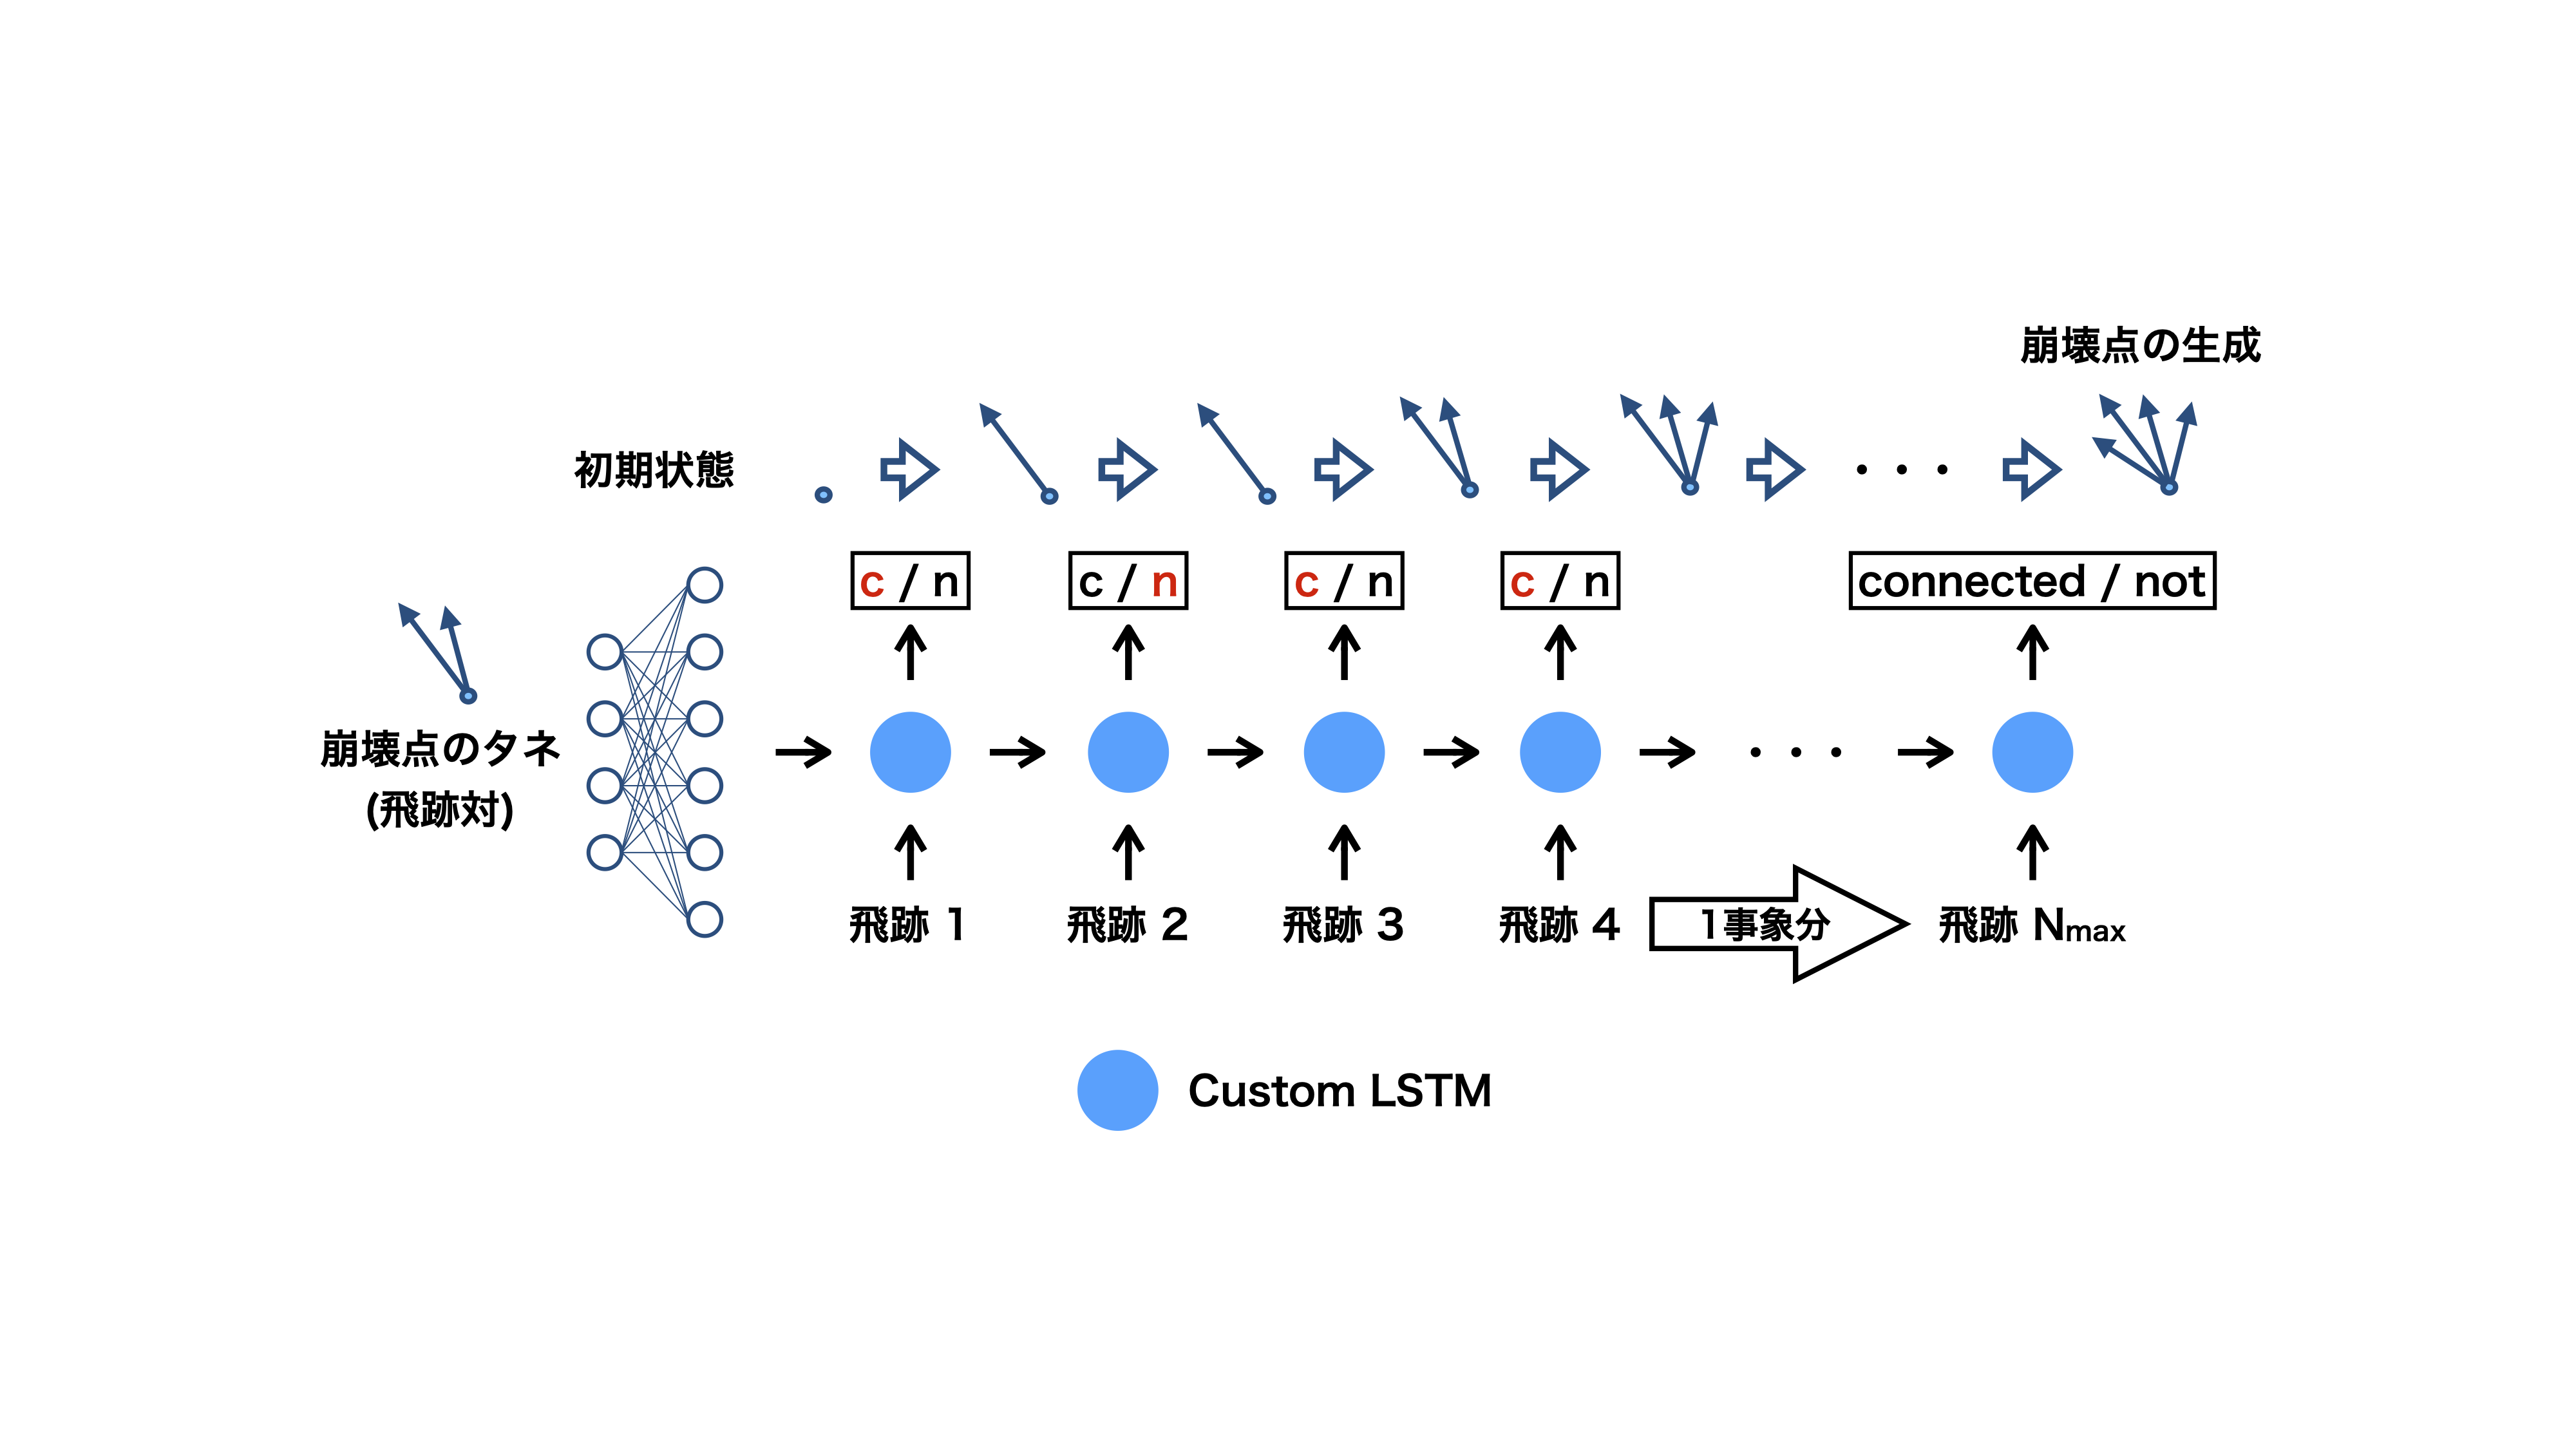
\includegraphics[trim = 0 80 0 0, width=1.0\textwidth]{Figure/3Networks/3-4-1-1SimpleVLSTM.png}
 \caption{独自のリカレントニューラルネットワーク構造を用いた崩壊点の生成}
 \label{3-4-1-1SimpleVLSTM}
\end{figure}

自然な発想として、今、飛跡について1事象分 (系列) の全ての情報を持っている為、エンコーダー・デコーダーモデルとすることで、その事象についての情報 (コンテキスト) を活用することができる。
更に、エンコーダー・デコーダーモデルの間にAttentionを組み込むことも同様に自然な発想である。
その様なネットワークを図\ref{3-4-1-2EncoderDecoderVLSTM}に示す。
この図では上から飛跡が入力されており、崩壊点の種である飛跡対は上部左右と左下から入力されている。
上部がエンコーダー部、下部がデコーダ部である。
個々の基本的な構造は図\ref{3-4-1-1SimpleVLSTM}と同一であるが、エンコーダー部には双方向リカレントニューラルネットワークを採用している。
また、デコーダー部では独自のリカレントニューラルネットワークの構造を更に拡張し、エンコーダー部の出力を初期状態の一つとしてAttentionに対応させたネットワークを使用している。
詳細は次項\ref{Net:VLSTM:DetailedStructureofVLSTM}にて述べる。

Attentionを組み込むことによって、デコーダー部の"ある"飛跡はエンコーダー部によって抽出された飛跡の情報に任意の注意を払って、1事象分の情報を取得することになる。
エンコーダー・デコーダーモデルに拡張しても、このネットワークの基本構造がリカレントニューラルネットワークであることに変わりがない為、デコーダー部の飛跡の本数を任意に変えることが可能である。

\begin{figure}[h]
 \centering
 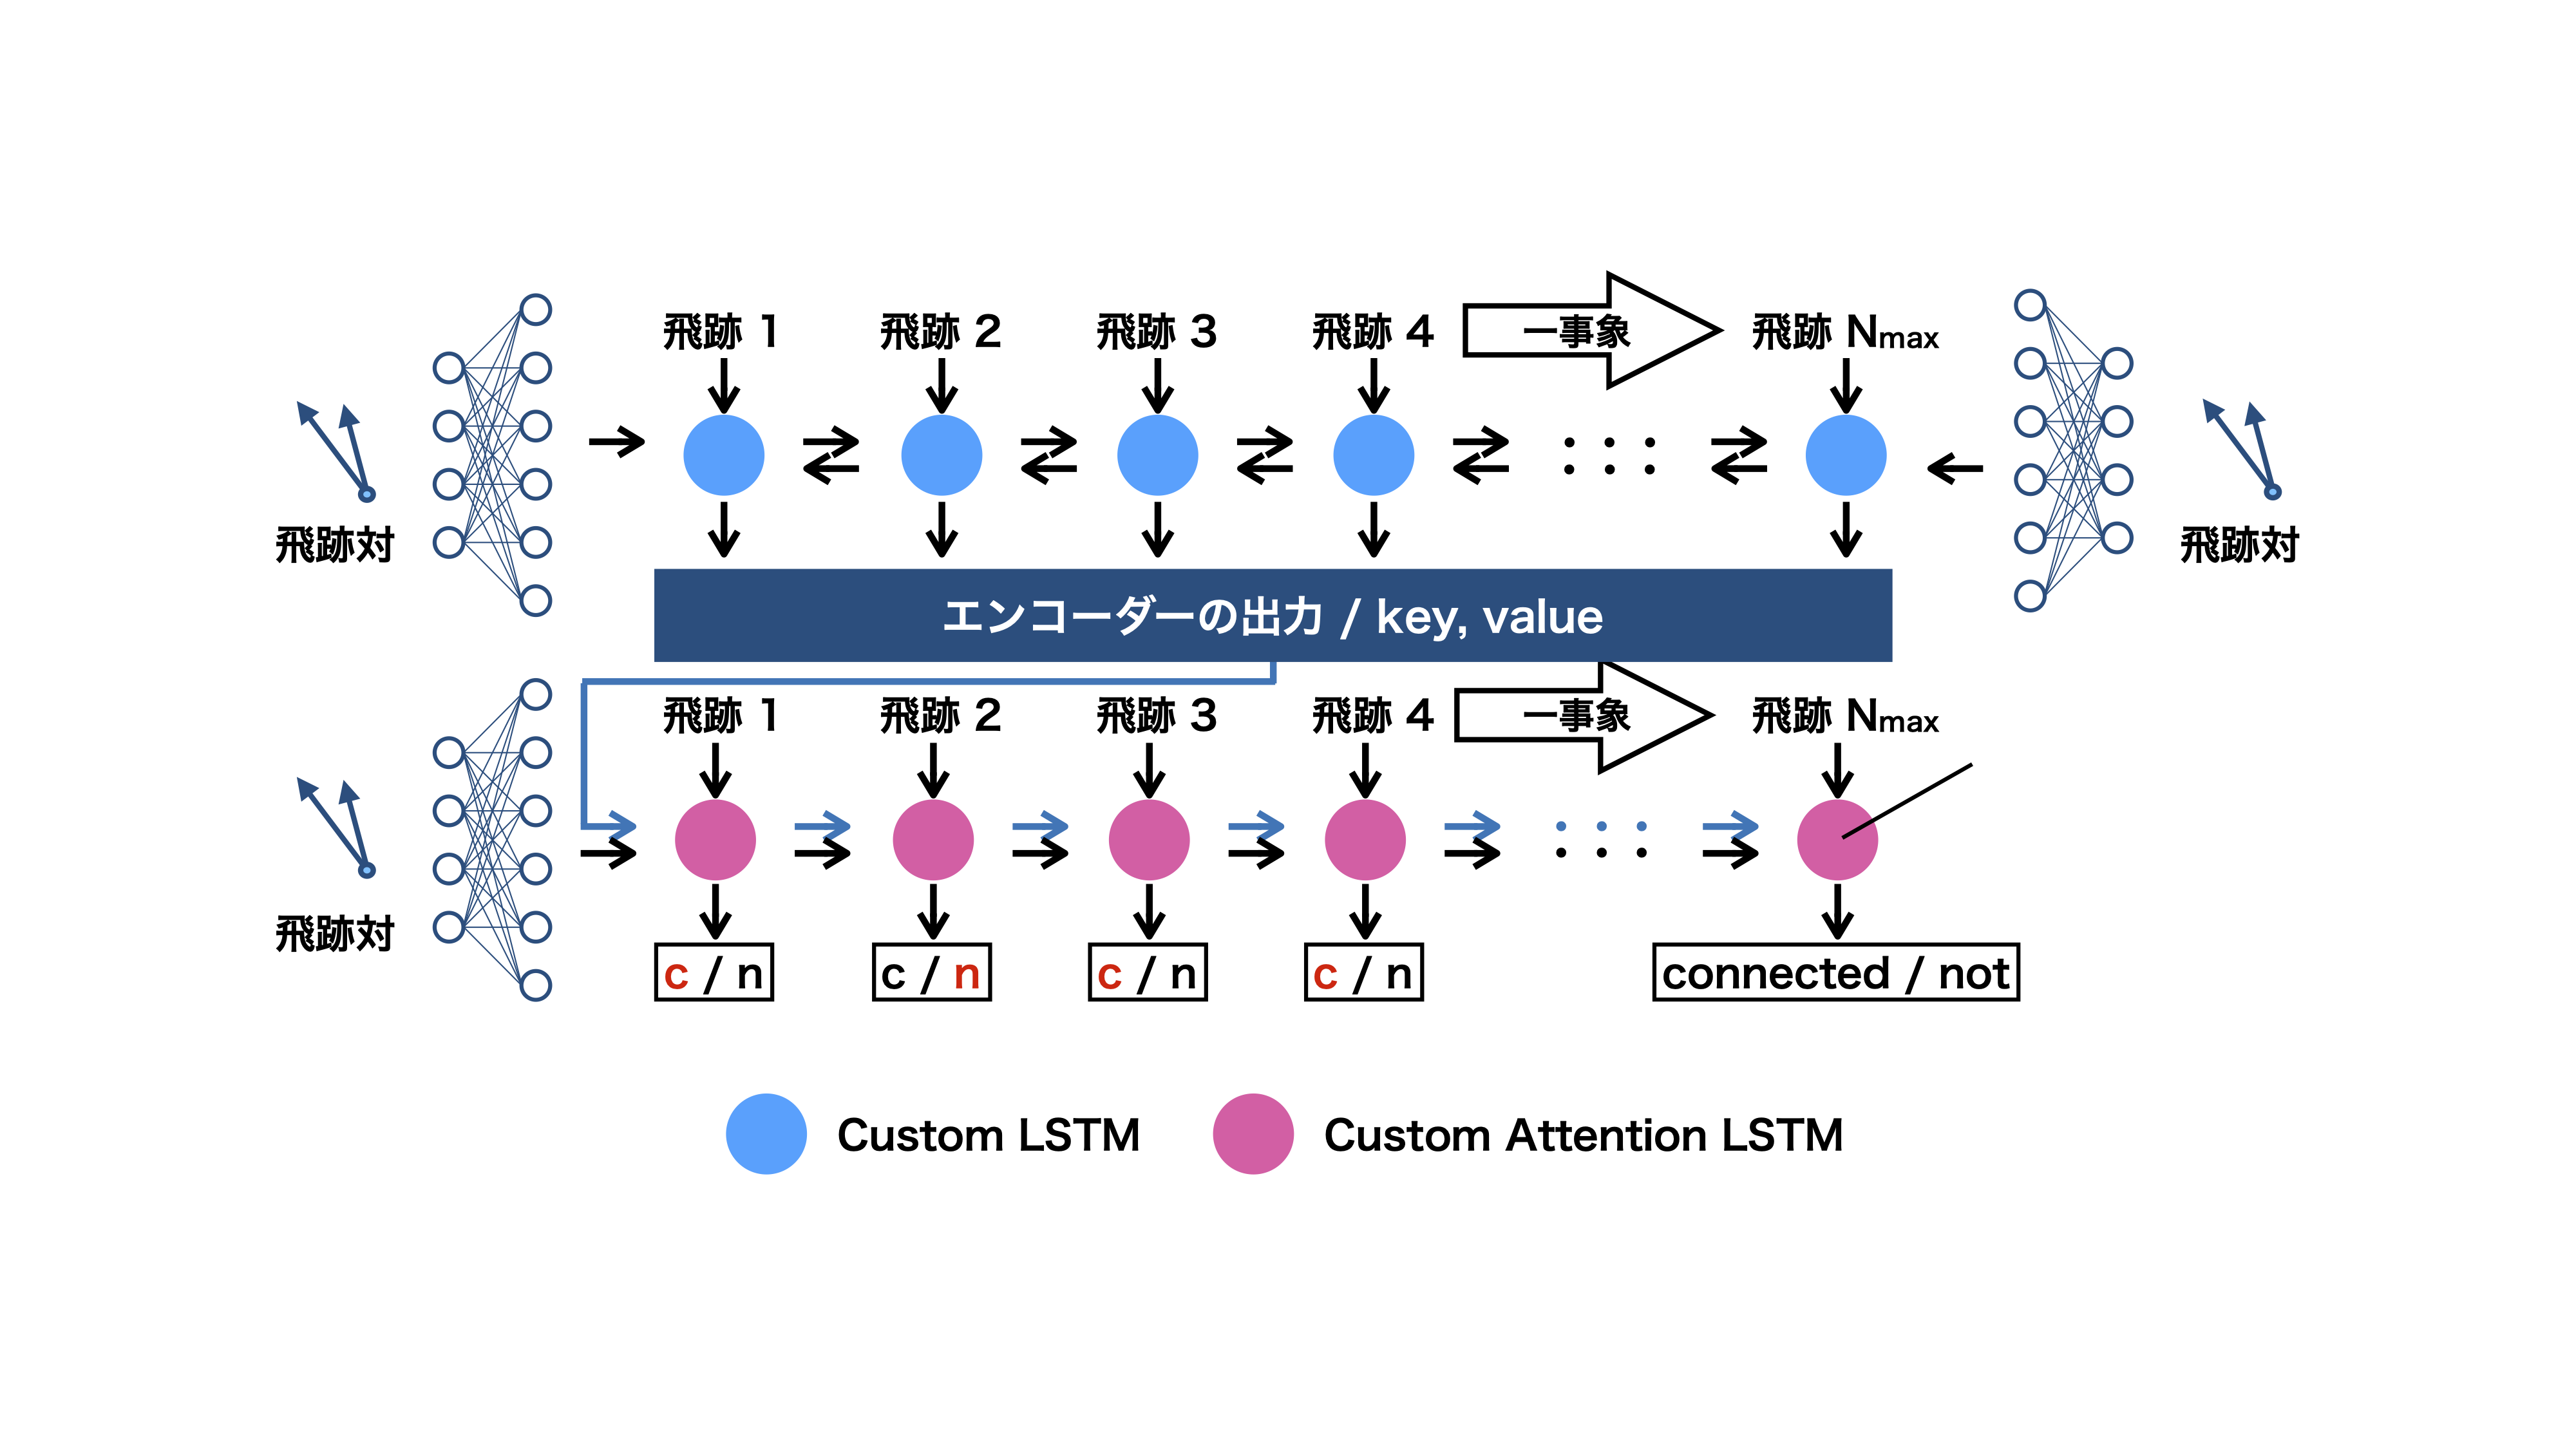
\includegraphics[trim = 0 80 0 0, width=1.0\textwidth]{Figure/3Networks/3-4-1-2EncoderDecoderVLSTM.png}
 \caption{Attentionを用いたエンコーダー・デコーダーモデルへの拡張}
 \label{3-4-1-2EncoderDecoderVLSTM}
\end{figure}

\begin{figure}[h]
 \centering
 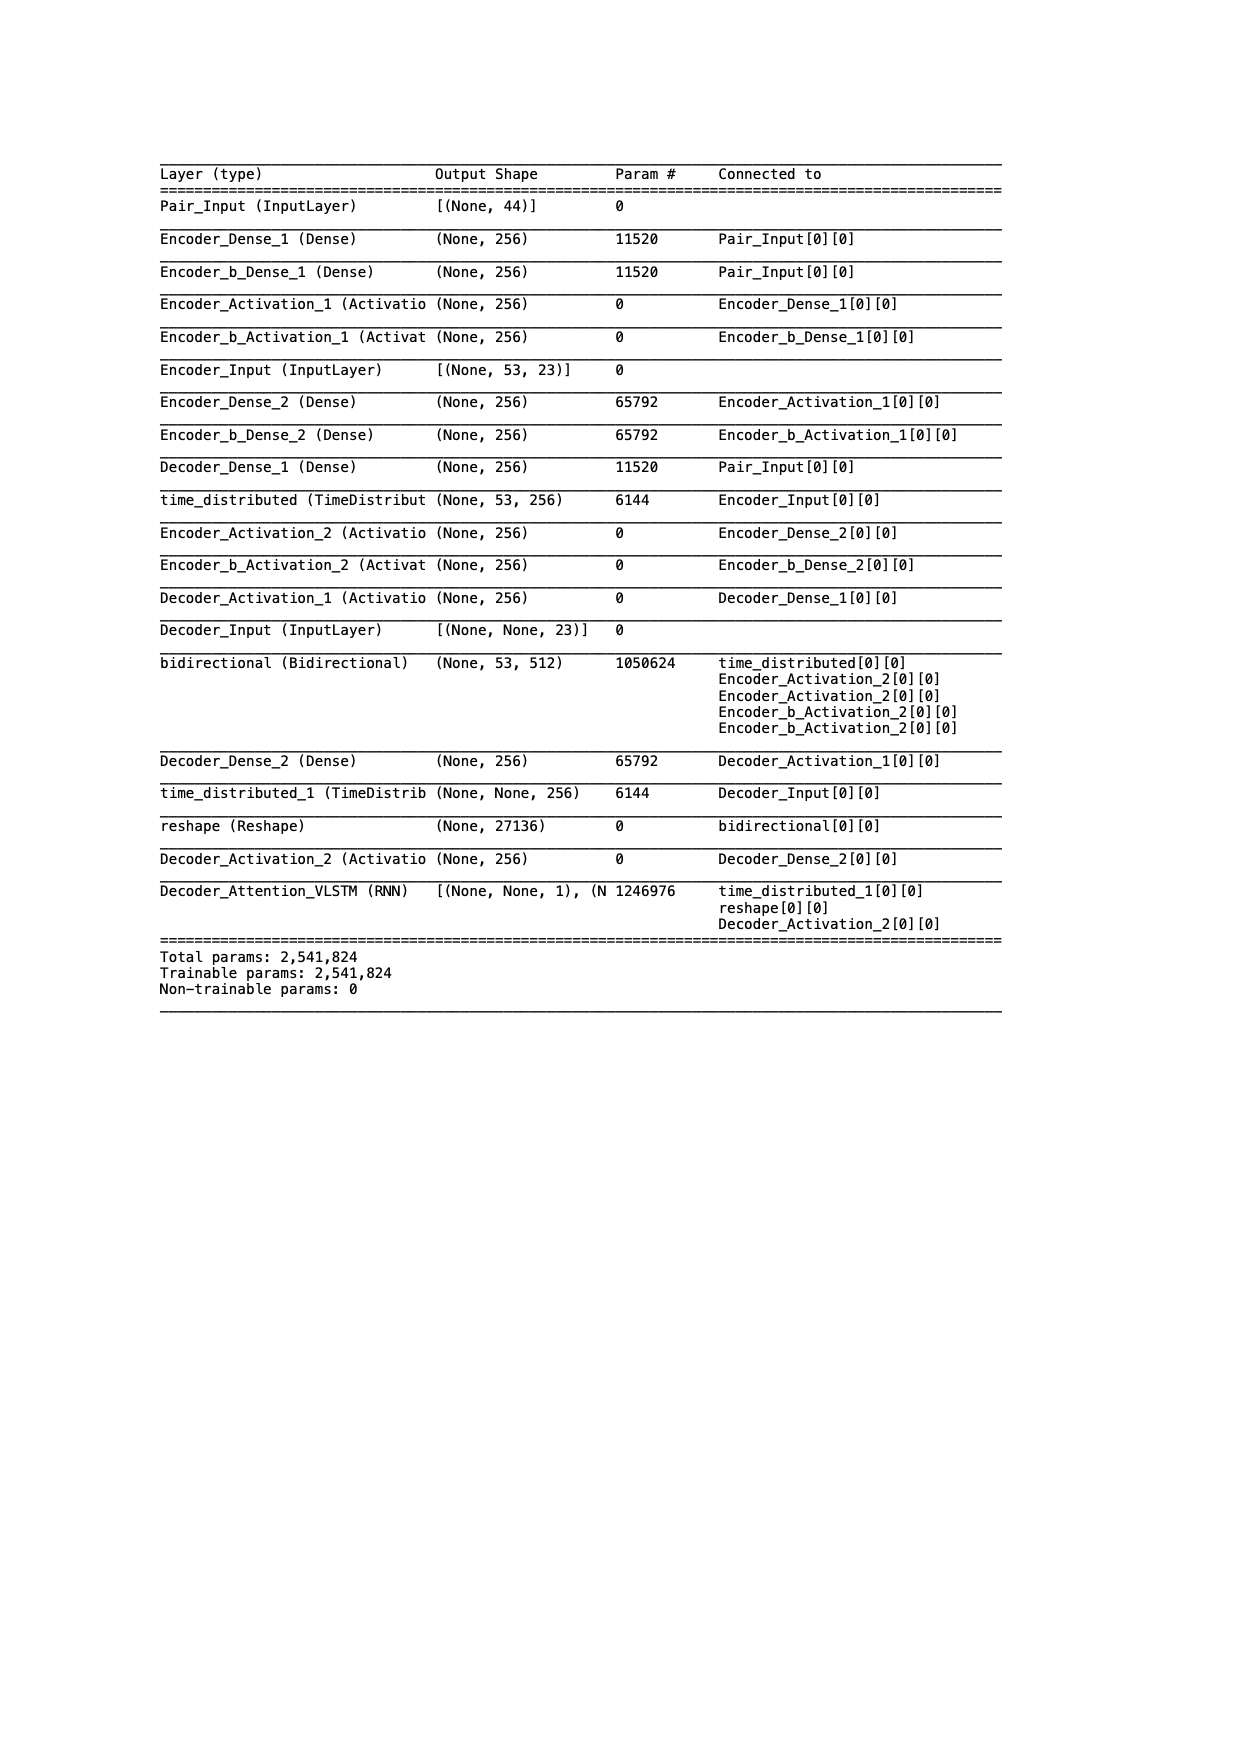
\includegraphics[trim = 75 300 125 0, width=0.9\textwidth]{Figure/3Networks/3-4-1-3VLSTMSummary.png}
 \caption{エンコーダー・デコーダーモデルにおける各種パラメーターの出力}
 \label{3-4-1-3VLSTMSummary}
\end{figure}


%%%%%%%%%%%%%%%%%%%%%%%%%%%%%%%%%%%%%%%%%%%%%%%%%%%%%%%%%%%%%%%%%%%%%%%%
\subsection{ネットワークの詳細な構造} \label{Net:VLSTM:DetailedStructureofVLSTM}

\begin{figure}[h]
 \centering
 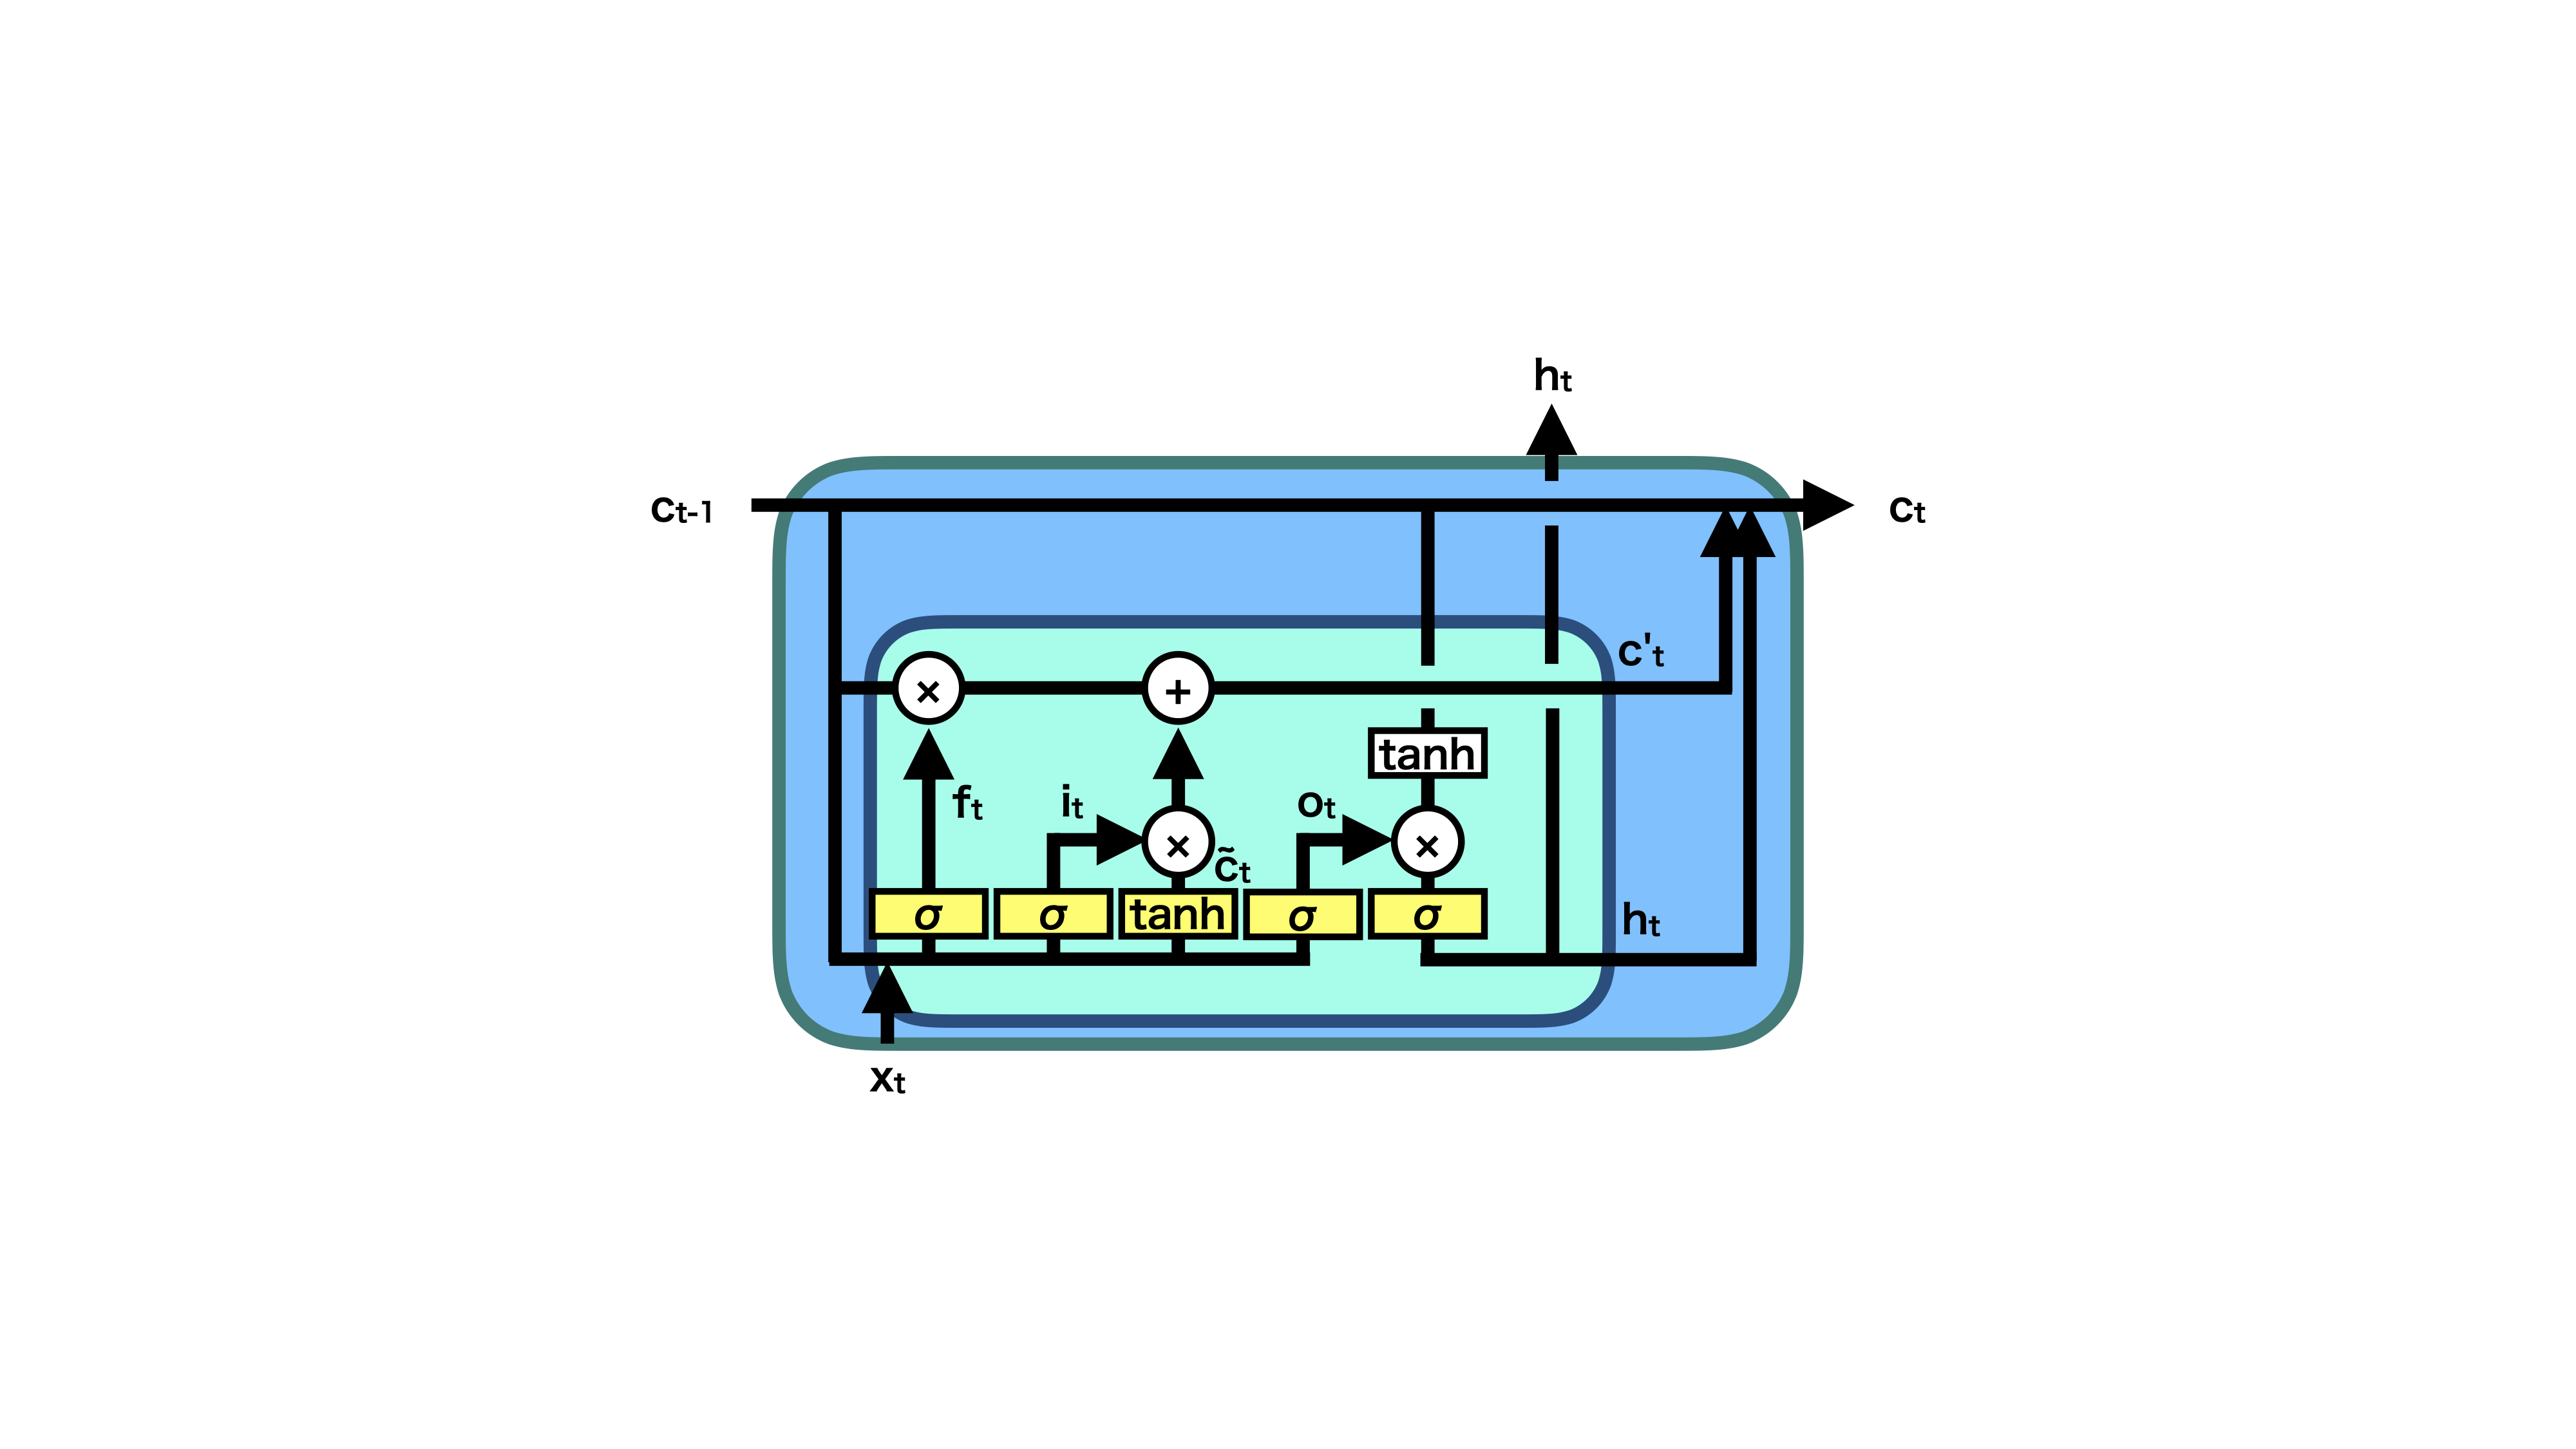
\includegraphics[width=0.9\textwidth]{Figure/3Networks/3-4-2-1VLSTMStructure.png}
 \caption{自作リカレントニューラルネットワークの構造}
 \label{3-4-2-1VLSTMStructure}
\end{figure}

\begin{figure}[h]
 \centering
 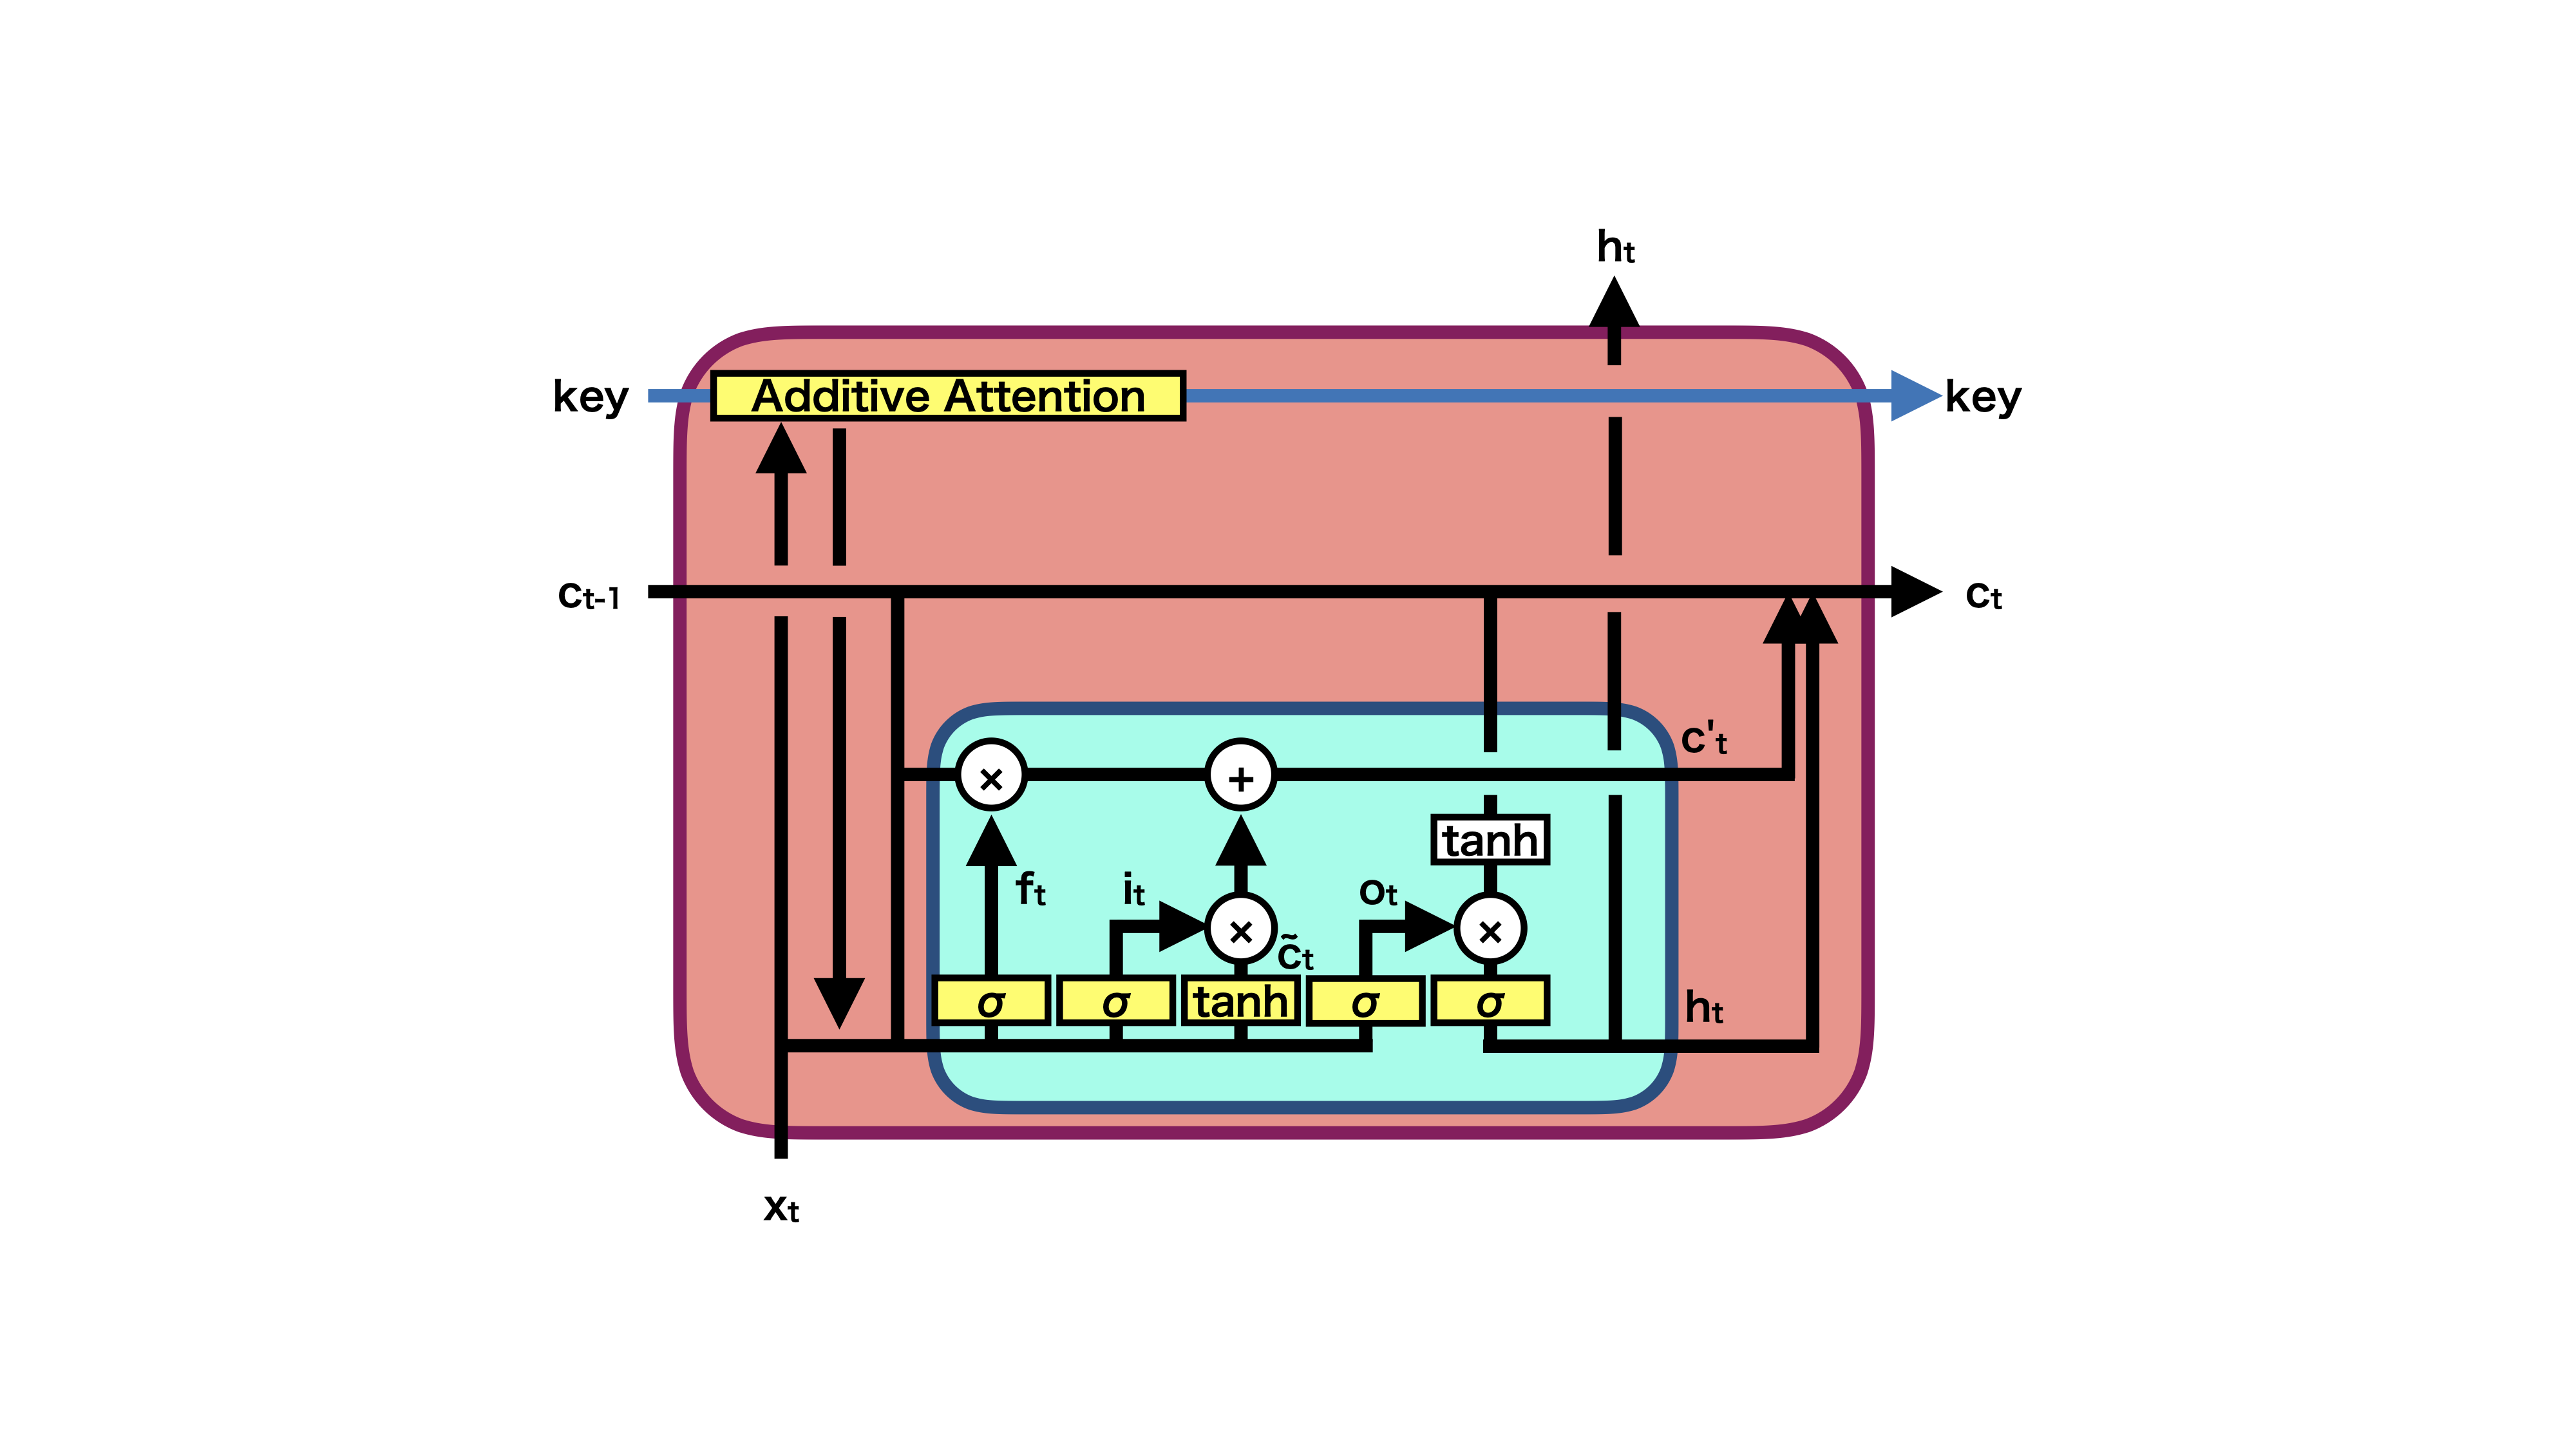
\includegraphics[width=0.9\textwidth]{Figure/3Networks/3-4-2-2AttentionVLSTM.png}
 \caption{Attentionを組み込んだ自作リカレントニューラルネットワークの構造}
 \label{3-4-2-2AttentionVLSTM}
\end{figure}


%%%%%%%%%%%%%%%%%%%%%%%%%%%%%%%%%%%%%%%%%%%%%%%%%%%%%%%%%%%%%%%%%%%%%%%%
\subsection{ネットワークの学習と戦略} \label{Net:VLSTM:TrainingandStrategyofVLSTM}

訓練データ\\
ゼロパディング

飛跡順のシャッフル

%%%%%%%%%%%%%%%%%%%%%%%%%%%%%%%%%%%%%%%%%%%%%%%%%%%%%%%%%%%%%%%%%%%%%%%%
\subsection{ネットワークの性能} \label{Net:VLSTM:PerformanceofVLSTM}

ハイパーパラメータ・チューニング\\

事象についての情報による変化\\

Attention weight\\

bb, ccデータセット









